\section{Audio Amplification Modules \& Speakers}

An audio module is an electronic device designed to amplify and process audio signals, allowing for the playback of sound in various applications. Speakers are transducers that convert electrical energy into sound energy, enabling us to hear audio signals. Together, audio modules and speakers create a complete audio playback system, necessary for applications ranging from personal electronics to professional sound systems.

\subsection{Speakers}

Speakers are devices that convert electrical signals into sound waves. They are classified into various types based on their design and application. Two common types of speakers include:

\begin{itemize}
	\item \textbf{Dynamic Speakers}: These are the most common type, using a voice coil and magnet to produce sound.
	\item \textbf{Subwoofers}: Specialized speakers designed to reproduce low-frequency sounds (bass), providing depth to the audio experience.
\end{itemize}

\subsection{Audio Modules}

Audio modules are compact devices designed to amplify audio signals and can include additional features like Bluetooth connectivity, equalization, and noise reduction. Some notable audio modules include:

\begin{figure}[h!]
	\centering
	\begin{subfigure}[b]{0.22\textwidth}
		\centering
		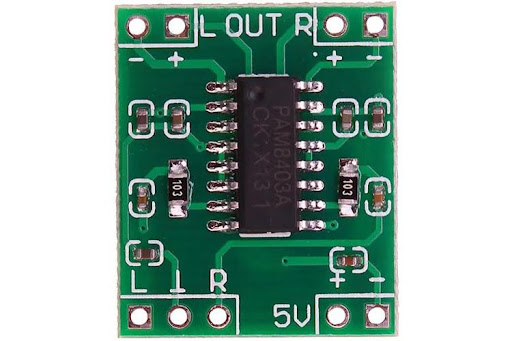
\includegraphics[width=\textwidth]{assets/ch2/PAM8403}
		\caption{}
		\label{fig:pam8403}
	\end{subfigure}
	\hfill
	\begin{subfigure}[b]{0.22\textwidth}
		\centering
		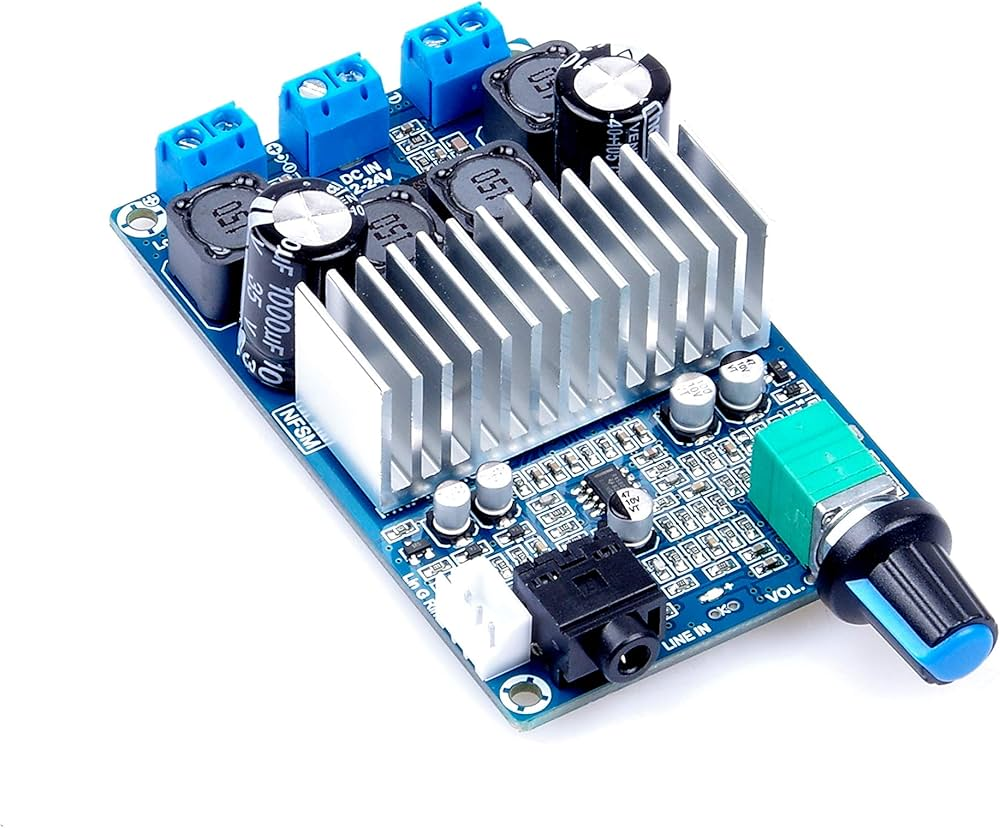
\includegraphics[width=\textwidth]{assets/ch2/TPA3116D2}
		\caption{}
		\label{fig:tpa3116d2}
	\end{subfigure}
	\hfill
	\begin{subfigure}[b]{0.22\textwidth}
		\centering
		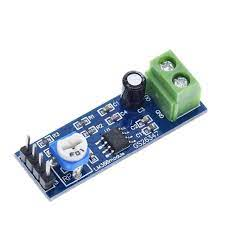
\includegraphics[width=\textwidth]{assets/ch2/LM386}
		\caption{}
		\label{fig:lm386}
	\end{subfigure}
	\hfill
	\begin{subfigure}[b]{0.22\textwidth}
		\centering
		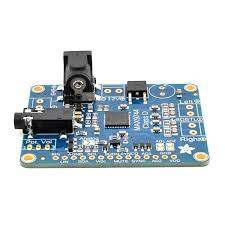
\includegraphics[width=\textwidth]{assets/ch2/MAX9744}
		\caption{}
		\label{fig:max9744}
	\end{subfigure}
	\caption{Audio Amplification Modules: (a) PAM8403, (b) TPA3116D2, (c) LM386, and (d) MAX9744.}
	\label{fig:audio_modules}
\end{figure}

\begin{itemize}
	\item \textbf{PAM8403}: A popular audio amplifier module known for its efficiency and compact size, suitable for small audio projects.
	
	
	\item \textbf{TPA3116D2}: A powerful audio amplifier capable of delivering higher output power, often used in larger audio systems.
	
	
	
	\item \textbf{LM386}: A low-power audio amplifier that is easy to use and perfect for basic applications.
	
	
	\item \textbf{MAX9744}: A high-efficiency audio amplifier designed for demanding audio applications, providing high-quality sound output.
	
	
\end{itemize}
